\documentclass[tocnopagenum]{thesis-ekf}
%a4paper, 12pt, 1.5-es sortávolság, margók
\usepackage[T1]{fontenc}
\PassOptionsToPackage{defaults=hu-min}{magyar.ldf}
\usepackage[magyar]{babel}
\usepackage{mathtools,amssymb,amsthm,pdfpages}
\footnotestyle{rule=fourth}
\usepackage{comment}

\newtheorem{tetel}{Tétel}[chapter]
\theoremstyle{definition}
\newtheorem{definicio}[tetel]{Definíció}
\theoremstyle{remark}
\newtheorem{megjegyzes}[tetel]{Megjegyzés}

\begin{document}
	\institute{Matematikai és Informatikai Intézet}
	\title{Interfész megoldások imperatív és OOP nyelvek közötti kapcsolattartásra}
	\author{Nagy-Tóth Bence\\Szak: Programtervező informatikus BSc\\Specializáció: Szoftverfejlesztő informatikus}
	\supervisor{Dr. Király Roland\\beosztás}
	\city{Eger}
	\date{2022}
	\maketitle
	\tableofcontents
	
	\chapter*{Bevezetés}
	\addcontentsline{toc}{chapter}{Bevezetés}
	\verb*|#TODO|: Bevezető szöveg...
	
	\chapter{Programozási nyelvekről általában}
	\section{A programozási nyelvek formális nyelvek?}
	\begin{definicio}
		Legyen $\mathbb{A} = \{a_1, a_2, ... a_n\}$ véges, nemüres ($ \mathbb{A} \neq \emptyset$) halmaz, ezt a nyelv ábécéjének, elemeit betűknek vagy jeleknek nevezzük. $\mathbb{A}$ halmaz elemeiből képezzük annak hatványait, ekkor 
		\begin{enumerate}
			\item $\mathbb{A} ^ {0}$ az üres szó ($\epsilon$) egyelemű halmazát, 
			\item $\mathbb{A} ^ {1} $ az egybetűs szavak halmazát (\,$\mathbb{A}^{1}\subseteq\mathbb{A}\wedge\mathbb{A}\subseteq\mathbb{A}^{1} \iff \mathbb{A}^{1}=\mathbb{A}$\,), 
			\item $\mathbb{A}^{2}$ a kétbetűs szavak halmazát jelenti, 
			\item $\mathbb{A}^{n}$ az n betűből álló szavak halmazát jelenti és így tovább.
		\end{enumerate}
	Jelölje $A^{*}=A^{0}\ \cup\ A^{1}\ \cup\ A^{2}\ \cup\ \dots\ \cup\  A^{n}$ az ábécé elemeiből képzett véges szavak/jelsorozatok halmazát (ezt $\mathbb{A}$ ábécé feletti univerzumnak hívjuk). Ekkor  $\mathbb{A}$-ból kirakható szavak $\mathbb{A}^{*}$ halmazának egy részhalmazát \textbf{formális nyelvnek} nevezzük. Szokásos még az $\mathbb{A}$ ábécé feletti formális nyelv megnevezés is. A hatványok a halmaz önmagával vett \emph{Descartes-szorzatait} jelentik.
	\cite{formnyelvek}
	\end{definicio}
	
	Fő különbségek formális és természetes nyelvek között:
	\begin{itemize}
		\item A formális nyelveket egy dedikált célra hozták létre az emberek, ezeket általában nem használják interperszonális (emberek közötti) kommunikációra. Ezzel szemben egy természetes nyelv (például az angol) egy emberi közösség jelkészletét rendszerezi.\\
		A C++ programozási nyelv például azért jöhetett létre Bjarne Stroustrup dán szoftverfejlesztő jóvoltából, mert a C - procedurális nyelv lévén - nem tette lehetővé többek között az objektum-orientált programozást, a memóriacímek helyett a biztonságosabb referenciák használatát. \cite{cpplang1}
		\item A formális nyelvek kulcsszavakból állnak. A természetes nyelvek építőkövei: fonémák (hangok, betűk), morfémák (szótövek, toldalékok), szavak, mondatok, bekezdések, szövegek.
		\item A természetes nyelvek fejlődhetnek spontán, emberi generációról generációra valamint tudatos módon (például nyelvújítás) egyaránt. A formális nyelvek alakulását egy tervezési fázis előzi meg, ekkor a nyelv szabályrendszerét lefektetik, tehát csak és kizárólag tudatos, mesterséges beavatkozással lehet megreformálni őket.
	\end{itemize} \cite{langvid1} \cite{langvid2}

	A fentiekből következően minden programozási nyelv formális nyelvnek számít. 
	
	2022-ben a legnépszerűbb programozási nyelvek:
	\begin{enumerate}
		\item JavaScript
		\begin{itemize}
			\item 1995, Brendan Eich fejlesztette a böngészési funkcionalitások kibővítése végett.
			\item web-, játék-, valamint mobilfejlesztés
			\item webszerverek felépítése
		\end{itemize}
		\item Python
		\begin{itemize}
			\item 1991, Guido Van Rossum tervezte egyszerűbb nyelvezet, a matematikai formulák illeszthetősége végett
			\item Backend-fejlesztés
			\item Data Science, automatizálás
			\item web scraping
		\end{itemize}
		\item HTML %valami más legyen ide
		\begin{itemize}
			\item webdokumentumok kezelése: JSON, XML, SVG
			\item weboldalak statikus (állandó) részeinek fejlesztése
		\end{itemize}
		\item CSS %valami más legyen ide
		\begin{itemize}
			\item 
			\item weboldalak formatervét, kinézetét, stílusát alakítja ki
			\item HTML mellett hívják segítségül
		\end{itemize}
		\item Java
		\begin{itemize}
			\item 1995, Sun Microsystems fejlesztése, alapötlet: olyan eszközök vezérlése, amelyek elférnek egy kézben
			\item E-commerce
			\item Finance
			\item App development
			\item it is often applied in industries such as banking, billing and the stock market.
			\item platformfüggetlen
		\end{itemize}
		\item SQL
		\begin{itemize}
			\item 1972, Donald D. Chamberlin és Raymond F. Boyce az IBM alkalmazásában, adattáblák egyszerűbb kezelésére
			\item adatbázisok kezelése, karbantartása
			\item Data Science\footnote{Az informatika, a matematikai statisztika és az üzleti elemzés metszetében álló tudományág, amely adatok összegyűjtésével, ezek elemzésével foglalkozik annak érdekében, hogy a vállalatok jobb üzleti döntéseket tudjanak meghozni ezek segítségével. \hyperref{https://qr.ae/pvlYmQ}{}{}{Forrás}}
		\end{itemize}
		\item Go
		\begin{itemize}
			\item 2009, a Google fejlesztői alakították ki, hogy megoldják a hatalmas szoftverrendszerekkel kapcsolatos problémákat
			\item rendszerek, hálózatok programozása
			\item hang- és videószerkesztés
			\item Big Data\footnote{Az informatika egyik tudományága, amely tömérdek mennyiségű, hagyományos számítógéppel nehezen kezelhető adatok tárolásával és feldolgozásával, ezek elemzésével foglalkozik.\hyperref{{https://www.youtube.com/watch?v=bAyrObl7TYE}}{}{}{Forrás}}
		\end{itemize}
		\item C
		\begin{itemize}
			\item 1970-es években Ken Thompson és Dennis Ritchie jóvoltából, Assembly-nél magasabb szintű (természetes nyelvezethez közelebb álló) nyelv kialakítása volt a célja
			\item beágyazott rendszerek illesztőprogramjai, vezérlőkódjai
			\item operációs rendszerek fejlesztése
			\item 3D videók szerkesztése
			\item alacsonyabb szintű a fentebb felsoroltaknál, ezért könnyebb optimalizálni
			\cite{clang1}
		\end{itemize}
	\end{enumerate}\cite{proglanguages1}\cite{proglanguages2}
	
	\chapter{Marshalling}
	\section{A}

	\begin{comment}
		Ezek később lesznek hasznosak
		\begin{tetel}
			Tétel szövege.
		\end{tetel}
		
		\begin{proof}
			Bizonyítás szövege.
		\end{proof}
		
		\begin{definicio}
			Definíció szövege.
		\end{definicio}
		
		\begin{megjegyzes}
			Megjegyzés szövege.
		\end{megjegyzes}
	\end{comment}
	
	\chapter*{Összegzés}
	\addcontentsline{toc}{chapter}{Összegzés}
	\verb*|#TODO|: Összefoglalás...
	\bibliographystyle{plain}
	\bibliography{references}
	
	% Aláírt, szkennelt nyilatkozat beillesztése a szakdolgozat végére
	%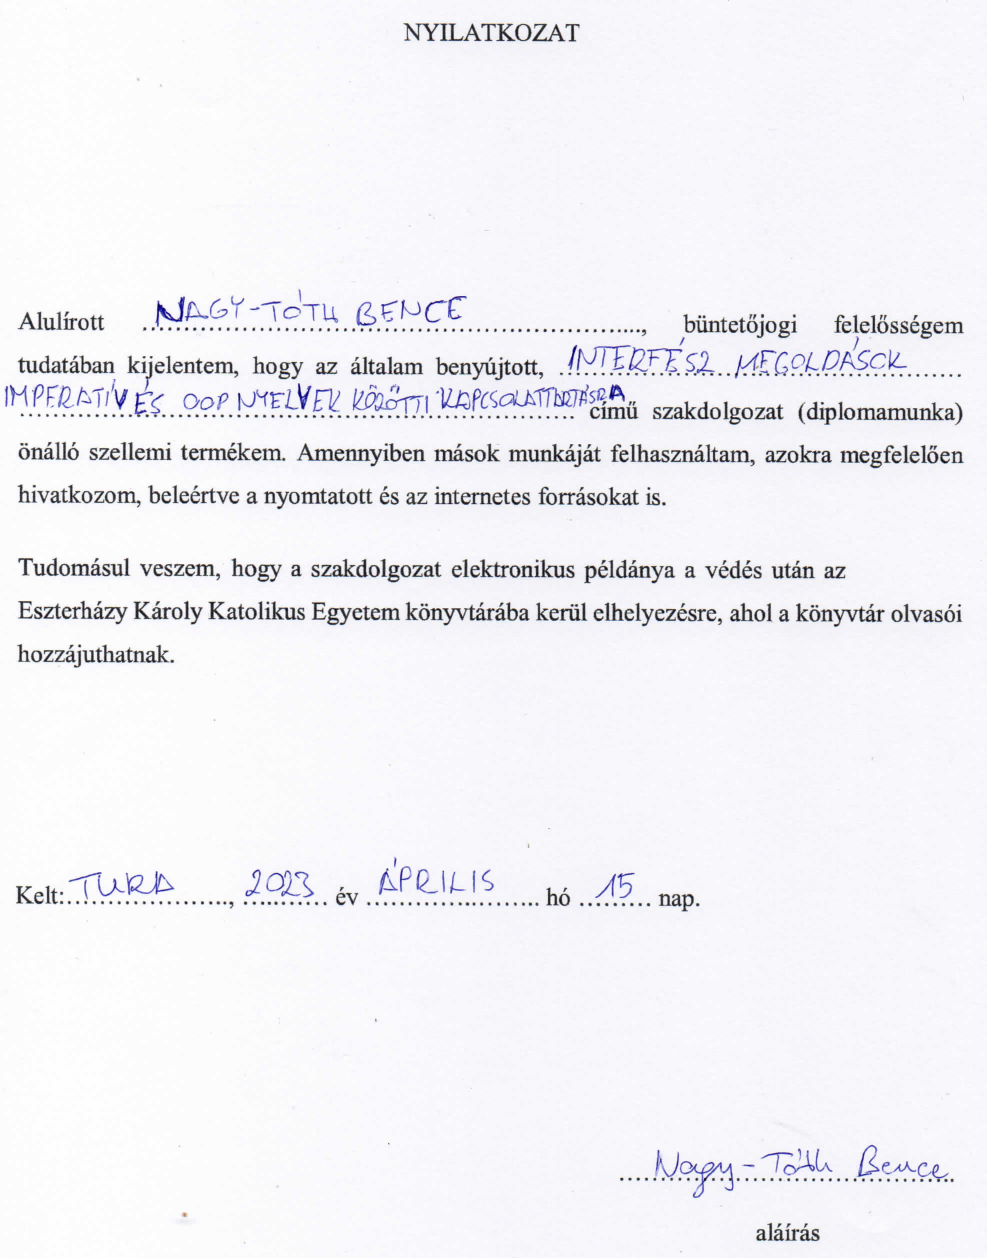
\includepdf{nyilatkozat.pdf}
\end{document}